\pagebreak
\section{Detailed Experiments}
\label{sec:detailedExperiments}

\subsection{Linear Probing}


\subsubsection{Add key:}
The order insert key to the Hash Table by Linear Probing is as follows: [one; 1], [two; 2], [three; 3], [four; 4], [five; 5], [one; 111], [two; 222]. The size of the Hash Table is 5. The Hash Table is shown in the figure below:

\begin{figure}[H]
	\centering
	\subfloat[\centering Add new]{{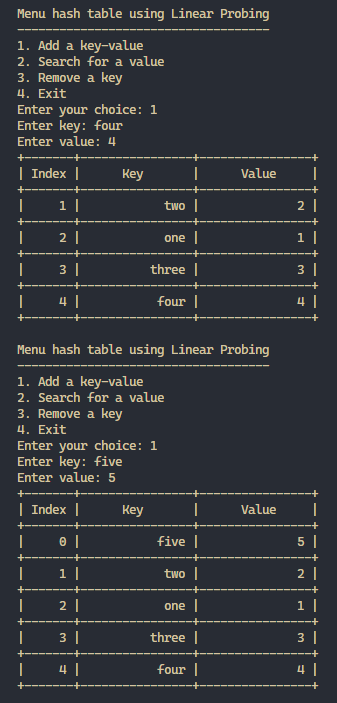
\includegraphics[width=7cm]{img/Linear/addnew.PNG} }}%
	\qquad
	\subfloat[\centering Update]{{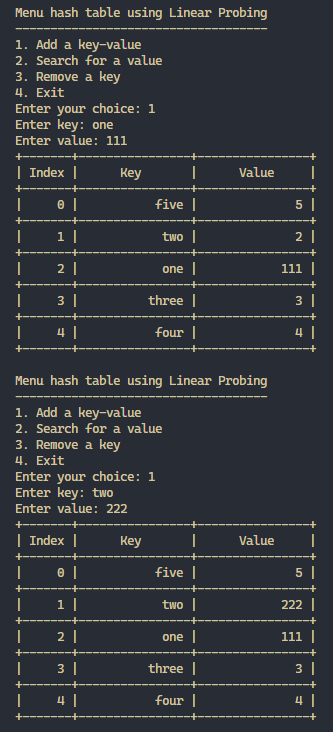
\includegraphics[width=7cm]{img/Linear/updateValue.PNG} }}%
	\caption{Add new by key by Linear Probing}%
\end{figure}

\subsubsection{Search key (Use the Hash Table added as above 3.1.1):}
\begin{figure}[H]
	\centering
	\subfloat[\centering Found]{{\includegraphics[width=7cm]{img/Linear/Found.PNG} }}%
	\qquad
	\subfloat[\centering Not Found]{{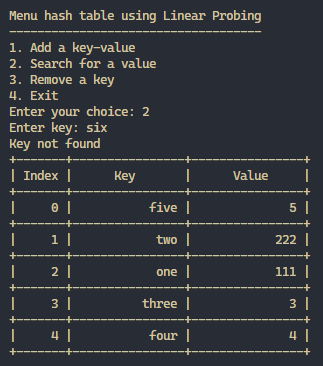
\includegraphics[width=7cm]{img/Linear/Not found.PNG} }}%
	\caption{Search value by key by Linear Probing (size=5)}%
\end{figure}

\subsubsection{Remove key (Use the Hash Table added as above 3.1.1):}
\begin{figure}[H]
	\centering
	\subfloat[\centering Removed]{{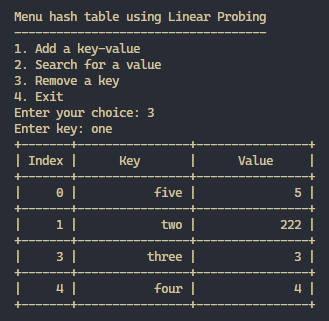
\includegraphics[width=7cm]{img/Linear/removed.PNG} }}%
	\qquad
	\subfloat[\centering Not Found]{{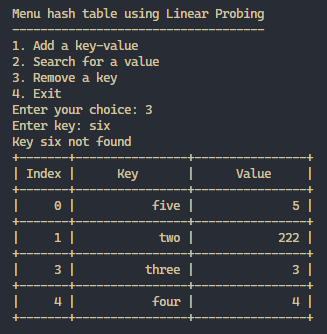
\includegraphics[width=7cm]{img/Linear/removeNotFound.PNG} }}%
	\caption{Remove value by key by Linear Probing}%
\end{figure}

\subsubsection{Experiments Linear Probing and Linear Search Algorithms}
\begin{figure}[H]
	\centering
	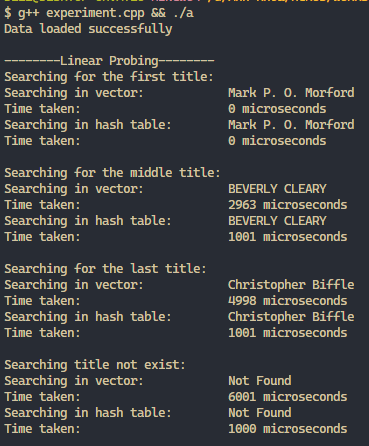
\includegraphics[width=0.7\linewidth]{img/Linear/Compare.PNG}
	\caption{Compare time Linear Probing Search and Linear Search Algorithms}
\end{figure}

\begin{itemize}
	\item The time complexity of Linear Probing Search is O(n)
	\item The time complexity of Linear Search Algorithms is O(n).
\end{itemize}
But in the most cases, using Linear Probing Search in Hash Table is faster than using Linear Search Algorithms in normal vector.

\pagebreak
\subsection{Quadratic Probing}


\subsubsection{Add key:}
The order insert key to the Hash Table by Quadratic Probing is as follows: [one; 1], [two; 2], [three; 3], [four; 4], [five; 5], [one; 111], [two; 222]. The size of the Hash Table is 5. But after added the key [three; 3], the size of the Hash Table is 10 by rehashing. However, this condition can be met even if there are still empty slots available, due to the nature of quadratic probing. The Hash Table is shown in the figure below:

\begin{figure}[H]
	\centering
	\subfloat[\centering Add new]{{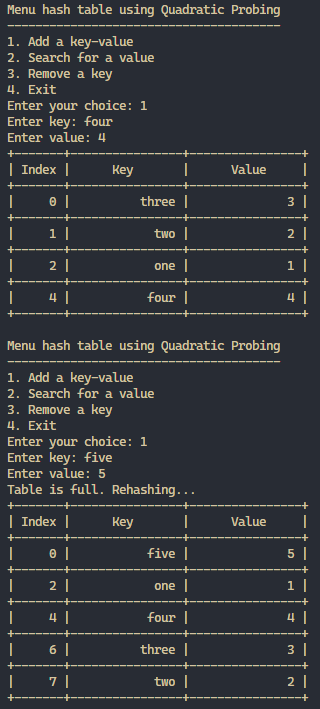
\includegraphics[width=7cm]{img/Quadratic/addnew.PNG} }}%
	\qquad
	\subfloat[\centering Update]{{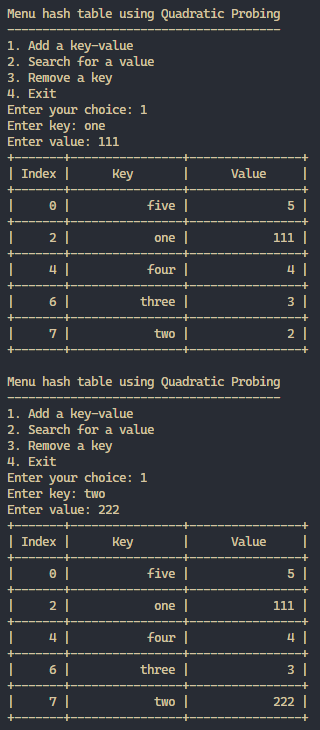
\includegraphics[width=7cm]{img/Quadratic/update.PNG}}}%
	\caption{Add new key by Quadratic Probing (size=5)}%
\end{figure}

\subsubsection{Search key (Use the Hash Table added as above 3.2.1):}
\begin{figure}[H]
	\centering
	\subfloat[\centering Found]{{\includegraphics[width=7cm]{img/Quadratic/Found.PNG} }}%
	\qquad
	\subfloat[\centering Not Found]{{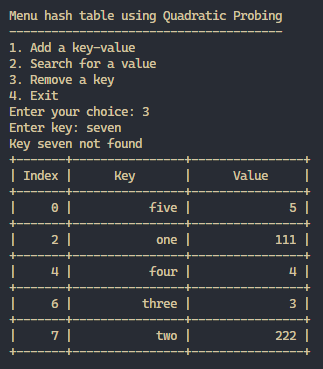
\includegraphics[width=7cm]{img/Quadratic/notFound.PNG} }}%
	\caption{Search value by key by Quadratic Probing (size=5)}%
\end{figure}

\subsubsection{Remove key (Use the Hash Table added as above 3.2.1):}
\begin{figure}[H]
	\centering
	\subfloat[\centering Removed]{{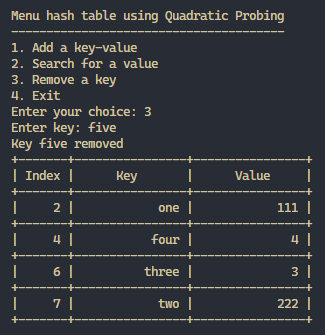
\includegraphics[width=7cm]{img/Quadratic/removed.PNG} }}%
	\qquad
	\subfloat[\centering Not Found]{{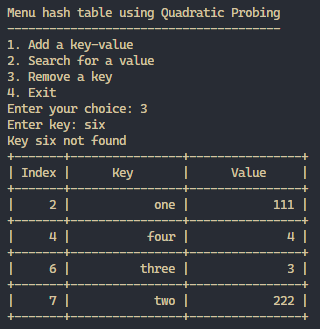
\includegraphics[width=7cm]{img/Quadratic/removeNotFound.PNG} }}%
	\caption{Remove value by key by Quadratic Probing}%
\end{figure}

\subsubsection{Experiments Quadratic Probing and Linear Search Algorithms}
\begin{figure}[H]
	\centering
	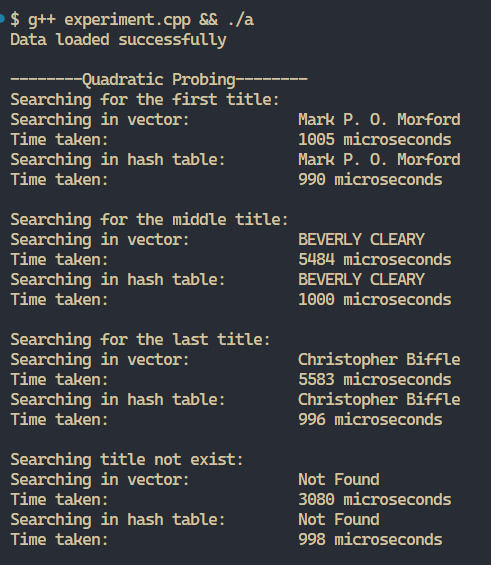
\includegraphics[width=0.7\linewidth]{img/Quadratic/compare.PNG}
	\caption{Compare time Quadratic Probing and Linear Search Algorithms}
\end{figure}

\begin{itemize}
	\item The time complexity of Quadratic Probing Search is O(n)
	\item The time complexity of Linear Search Algorithms is O(n).
\end{itemize}
But in the most cases, using Quadratic Probing Search in Hash Table is faster than using Linear Search Algorithms in normal vector.\\

\pagebreak
\subsection{Chaining using Linked List}

\subsubsection{Add key:}
The order insert key to the Hash Table by Chaining using Linked List is as follows: [one; 1], [two; 2], [three; 3], [four; 4], [five; 5], [one; 111], [two; 222]. The size of the Hash Table is 5. The Hash Table is shown in the figure below:

\begin{figure}[H]
	\centering
	\subfloat[\centering Add new]{{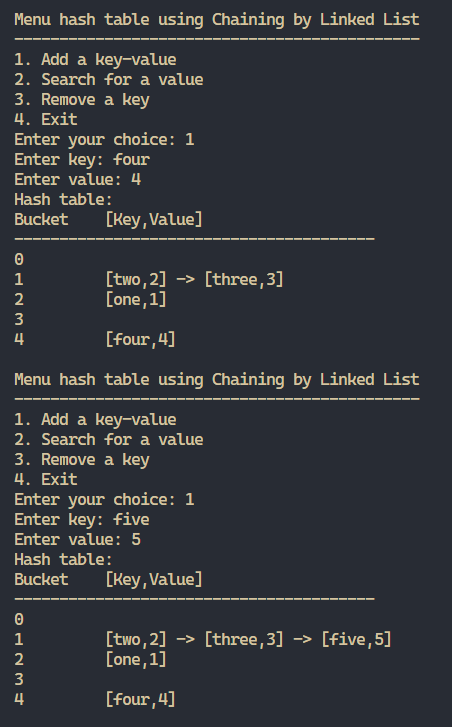
\includegraphics[width=7cm]{img/ChainingLinkedList/addnew.PNG} }}%
	\qquad
	\subfloat[\centering Update]{{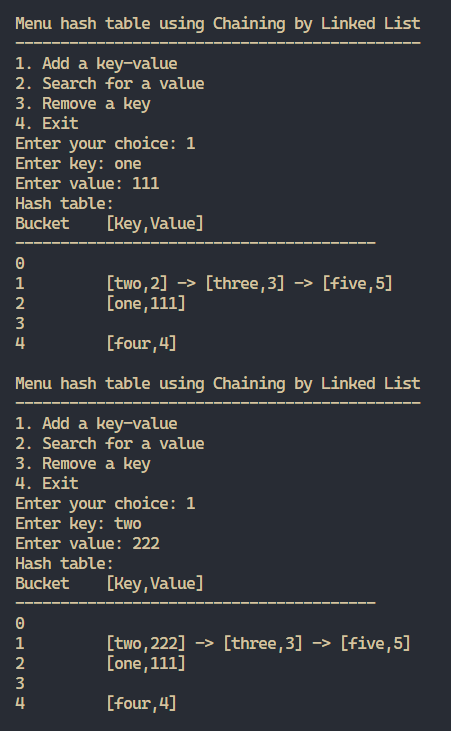
\includegraphics[width=7cm]{img/ChainingLinkedList/update.PNG} }}%
	\caption{Add new by key by Chaining using Linked List}%
\end{figure}

\subsubsection{Search key (Use the Hash Table added as above 3.3.1):}
\begin{figure}[H]
	\centering
	\subfloat[\centering Found]{{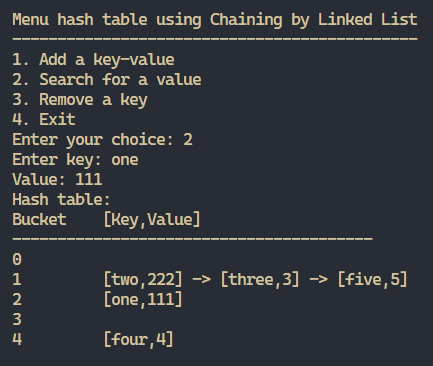
\includegraphics[width=7cm]{img/ChainingLinkedList/found.PNG} }}%
	\qquad
	\subfloat[\centering Not Found]{{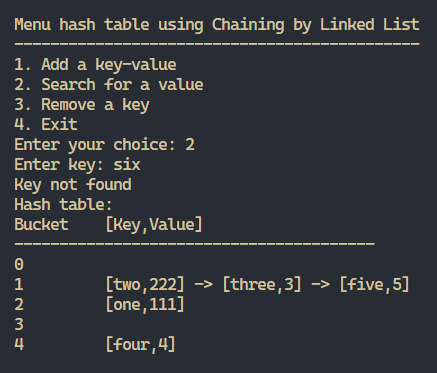
\includegraphics[width=7cm]{img/ChainingLinkedList/notfound.PNG} }}%
	\caption{Search value by key by Chaining using Linked List}%
\end{figure}

\subsubsection{Remove key (Use the Hash Table added as above 3.3.1):}
\begin{figure}[H]
	\centering
	\subfloat[\centering Removed]{{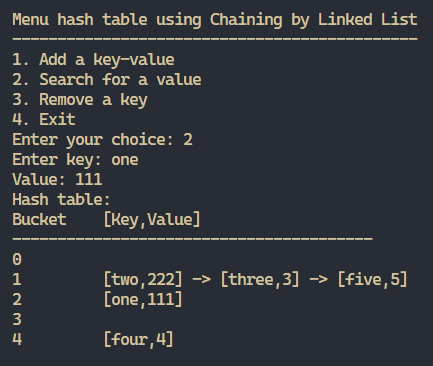
\includegraphics[width=7cm]{img/ChainingLinkedList/found.PNG} }}%
	\qquad
	\subfloat[\centering Not Found]{{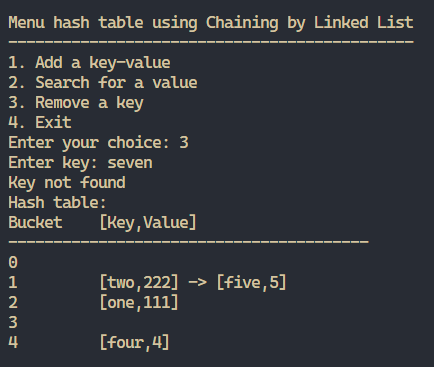
\includegraphics[width=7cm]{img/ChainingLinkedList/removeNotFound.PNG} }}%
	\caption{Remove value by key by Chaining Using Linked List}%
\end{figure}

\subsubsection{Experiments Chaining Using Linked List and Linear Search Algorithms}
\begin{figure}[H]
	\centering
	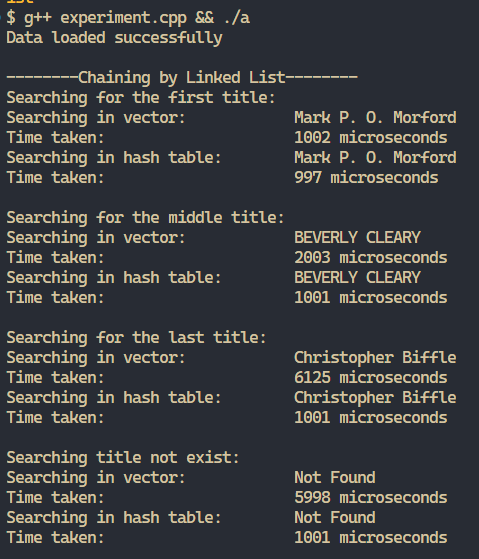
\includegraphics[width=0.7\linewidth]{img/ChainingLinkedList/compare.PNG}
	\caption{Compare time Chaining using Linked List Search and Linear Search Algorithms}
\end{figure}

\begin{itemize}
	\item The time complexity of Chaining using Linked List Search is O(n)
	\item The time complexity of Linear Search Algorithms is O(n).
\end{itemize}
But in the most cases, using Chaining using Linked List Search in Hash Table is faster than using Linear Search Algorithms in normal vector.

\pagebreak
\subsection{Chaining using AVL Tree}
\subsubsection{Add key:}
The order insert key to the Hash Table by Chaining using AVL Tree is as follows: [one; 1], [two; 2], [three; 3], [four; 4], [five; 5], [one; 111], [two; 222]. The size of the Hash Table is 5. The Hash Table is shown in the figure below:

\begin{figure}[H]
	\centering
	\subfloat[\centering Add new]{{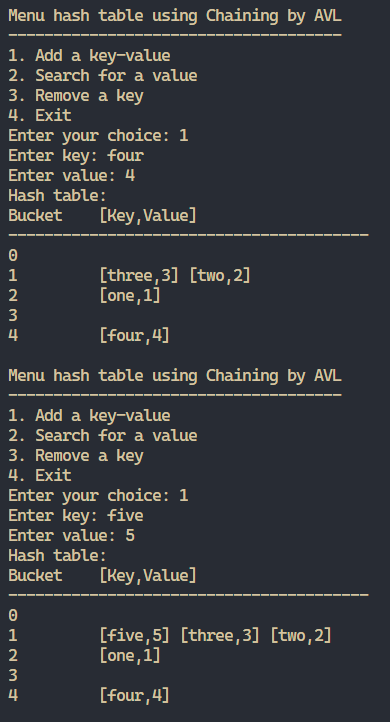
\includegraphics[width=7cm]{img/ChainingAVL/addnew.PNG} }}%
	\qquad
	\subfloat[\centering Update]{{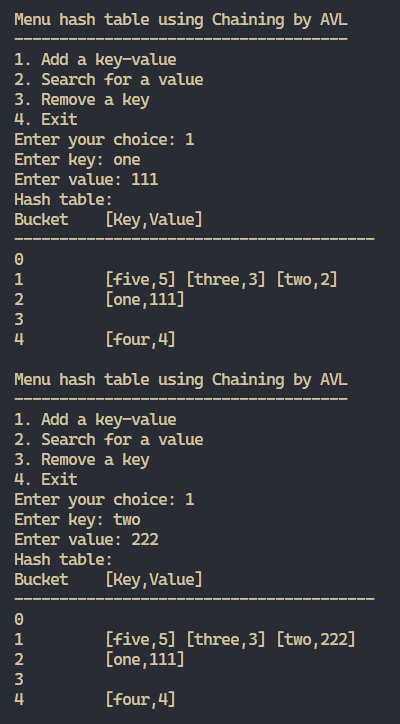
\includegraphics[width=7cm]{img/ChainingAVL/update.PNG} }}%
	\caption{Add new by key by Chaining using AVL Tree}%
\end{figure}

\subsubsection{Search key (Use the Hash Table added as above 3.4.1):}
\begin{figure}[H]
	\centering
	\subfloat[\centering Found]{{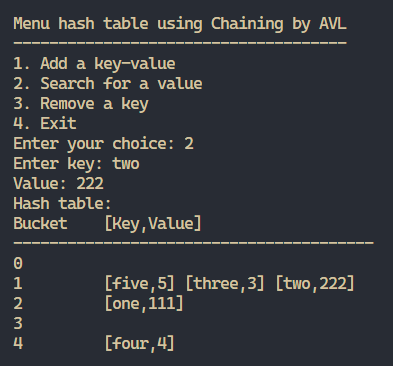
\includegraphics[width=7cm]{img/ChainingAVL/found.PNG} }}%
	\qquad
	\subfloat[\centering Not Found]{{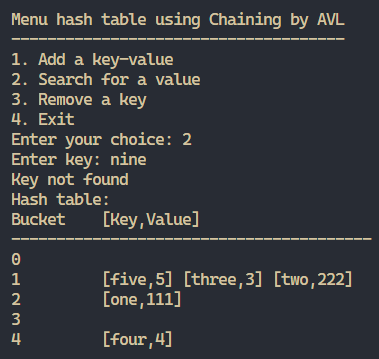
\includegraphics[width=7cm]{img/ChainingAVL/notfound.PNG} }}%
	\caption{Search value by key by CChaining Using AVL Tree}%
\end{figure}

\subsubsection{Remove key (Use the Hash Table added as above 3.4.1):}
\begin{figure}[H]
	\centering
	\subfloat[\centering Removed]{{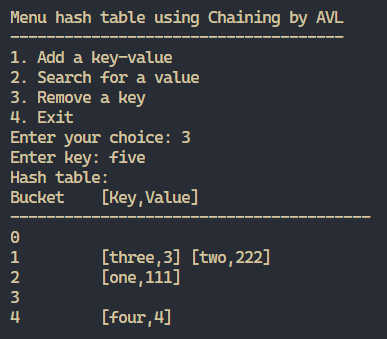
\includegraphics[width=7cm]{img/ChainingAVL/removed.PNG} }}%
	\qquad
	\subfloat[\centering Not Found]{{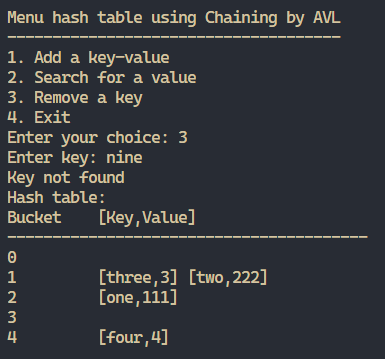
\includegraphics[width=7cm]{img/ChainingAVL/removeNotFound.PNG} }}%
	\caption{Remove value by key by Chaining Using AVL Tree}%
\end{figure}

\subsubsection{Experiments Chaining using AVL Tree and Linear Search Algorithms}
\begin{figure}[H]
	\centering
	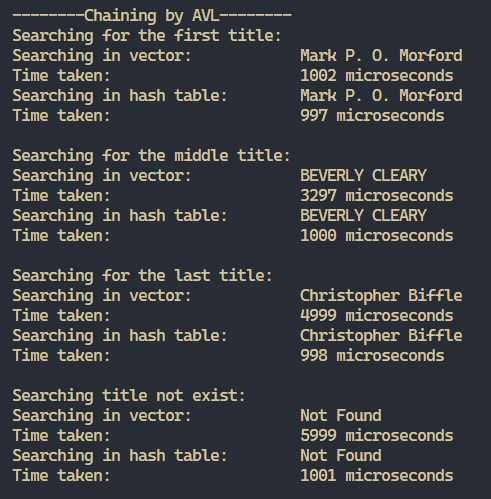
\includegraphics[width=0.7\linewidth]{img/ChainingAVL/compare.PNG}
	\caption{Compare time Chaining using AVL Tree Search and Linear Search Algorithms}
\end{figure}

\begin{itemize}
	\item The time complexity of Chaining using AVL Tree Search is O(logn)
	\item The time complexity of Linear Search Algorithms is O(n).
\end{itemize}
So in the most cases, using Chaining using AVL Tree Search in Hash Table is faster than using Linear Search Algorithms in normal vector.


\pagebreak
\subsection{Double Hashing}

\subsubsection{Add key:}
The order insert key to the Hash Table size = 5 by Double Hashing is as follows: [one; 1], [two; 2], [three; 3], [four; 4], [five; 5], [one; 111], [two; 222].The Hash Table is shown in the figure below:

\begin{figure}[H]
	\centering
	\subfloat[\centering Add new]{{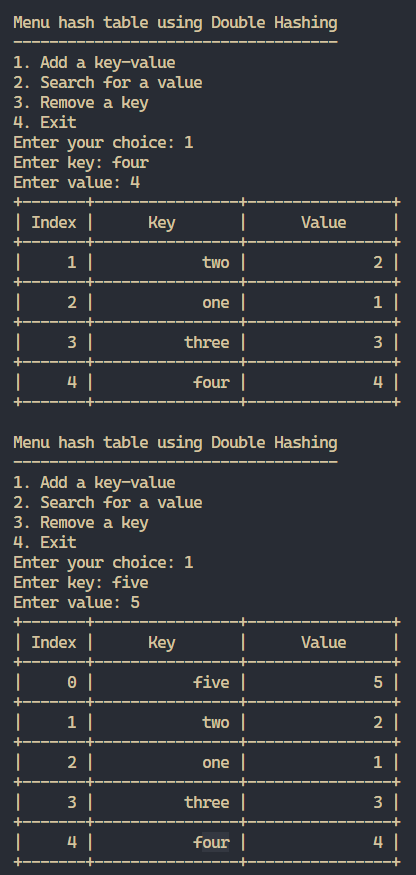
\includegraphics[width=7cm]{img/DoubleHash/addnew.PNG} }}%
	\qquad
	\subfloat[\centering Update]{{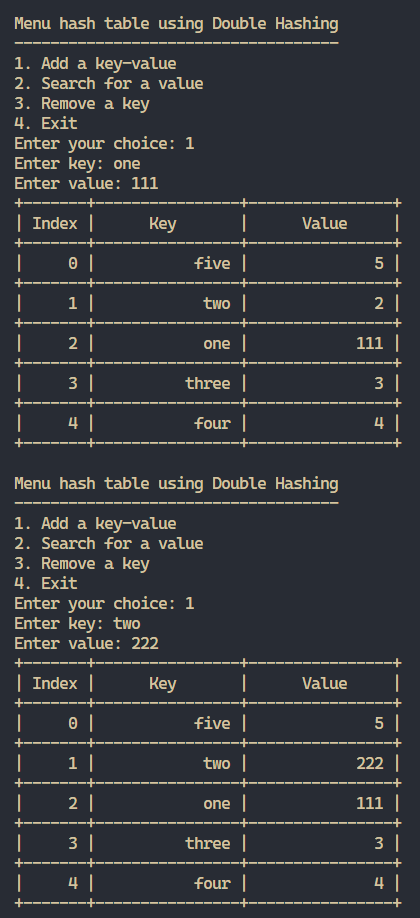
\includegraphics[width=7cm]{img/DoubleHash/update.PNG}}}%
	\caption{Add new key by Quadratic Probing (size=5)}%
\end{figure}

\subsubsection{Search key (Use the Hash Table added as above 3.5.1):}
\begin{figure}[H]
	\centering
	\subfloat[\centering Found]{{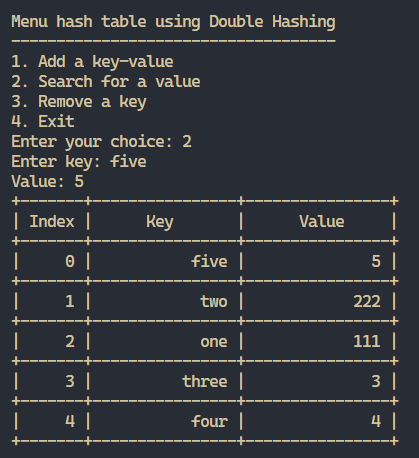
\includegraphics[width=7cm]{img/DoubleHash/found.PNG} }}%
	\qquad
	\subfloat[\centering Not Found]{{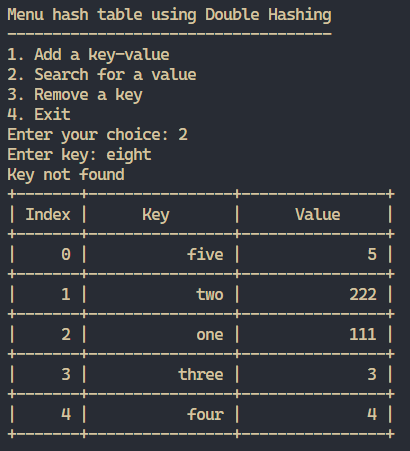
\includegraphics[width=7cm]{img/DoubleHash/notfound.PNG} }}%
	\caption{Search value by key by Quadratic Probing (size=5)}%
\end{figure}

\subsubsection{Remove key (Use the Hash Table added as above 3.5.1):}
\begin{figure}[H]
	\centering
	\subfloat[\centering Removed]{{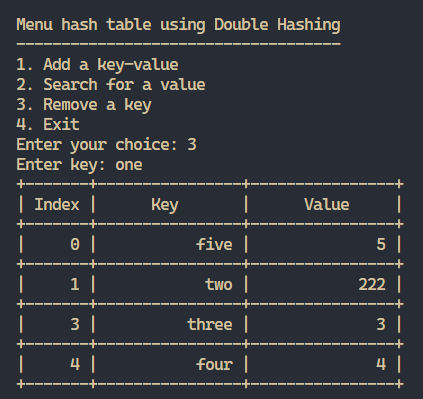
\includegraphics[width=7cm]{img/DoubleHash/removed.PNG} }}%
	\qquad
	\subfloat[\centering Not Found]{{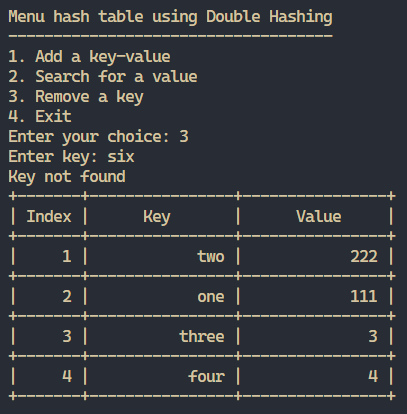
\includegraphics[width=7cm]{img/DoubleHash/removeNotFound.PNG} }}%
	\caption{Remove value by key by Double Hashing}%
\end{figure}

\subsubsection{Experiments Double Hashing and Linear Search Algorithms}
\begin{figure}[H]
	\centering
	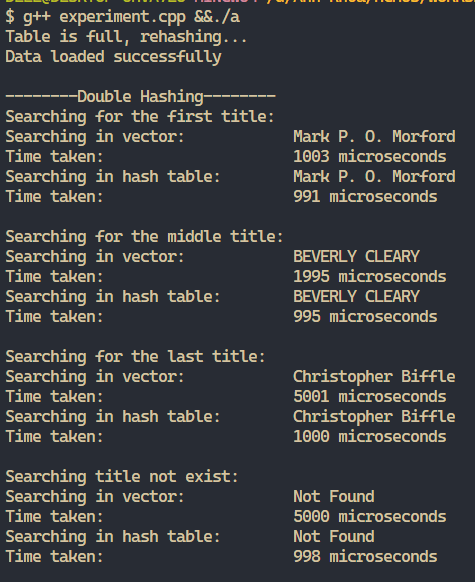
\includegraphics[width=0.7\linewidth]{img/DoubleHash/compare.PNG}
	\caption{Compare time Double Hashing Search and Linear Search Algorithms}
\end{figure}

\begin{itemize}
	\item The time complexity of Double Hashing Search is O(n)
	\item The time complexity of Linear Search Algorithms is O(n).
\end{itemize}
But in the most cases, using Double Hashing Search in Hash Table is faster than using Linear Search Algorithms in normal vector.\\

When run with large dataset, Hash Table by Double Hashing need to rehash because the condition \textbf{ if (i == capacity)} is used to determine if the table is full. However, this condition can be met even if there are still empty slots available, due to the nature of quadratic probing.
